\documentclass{article}
\usepackage{graphicx}
\usepackage{amsmath}
\usepackage[parfill]{parskip}
\usepackage{hyperref}
\graphicspath{ {./figures/} }

\title{COMP.SEC.220 Security Protocol\footnote{github --- \url{https://github.com/ancuongnguyen07/SecurityProtocol}}}
\author{Cuong Nguyen --- LAB 6}
\date{02/10/2022}

\begin{document}
    
\maketitle

\section*{Exercise 1 --- Creating a Dictionary}

\begin{figure}[!hpt]
    \centering
    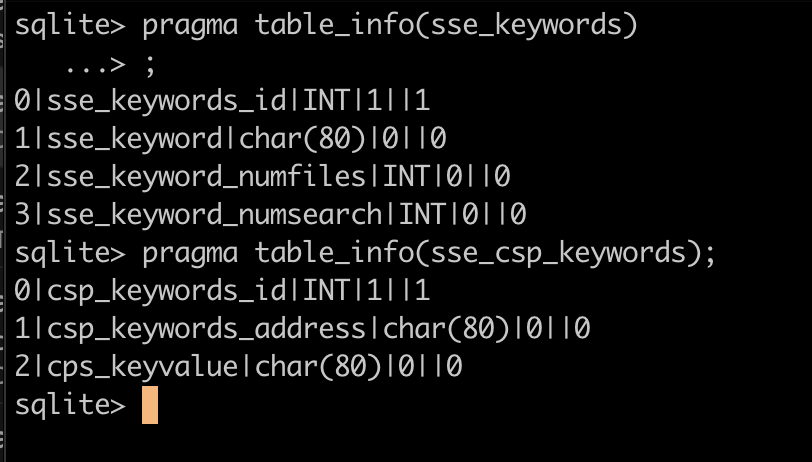
\includegraphics[height=\textheight,width=\textwidth,
                    keepaspectratio]{tables_info.png}
    \caption{Info of two tables: \emph{sse\_csp\_keywords} and
    \emph{sse\_keywords}.}
\end{figure}

\begin{figure}[!hpt]
    \centering
    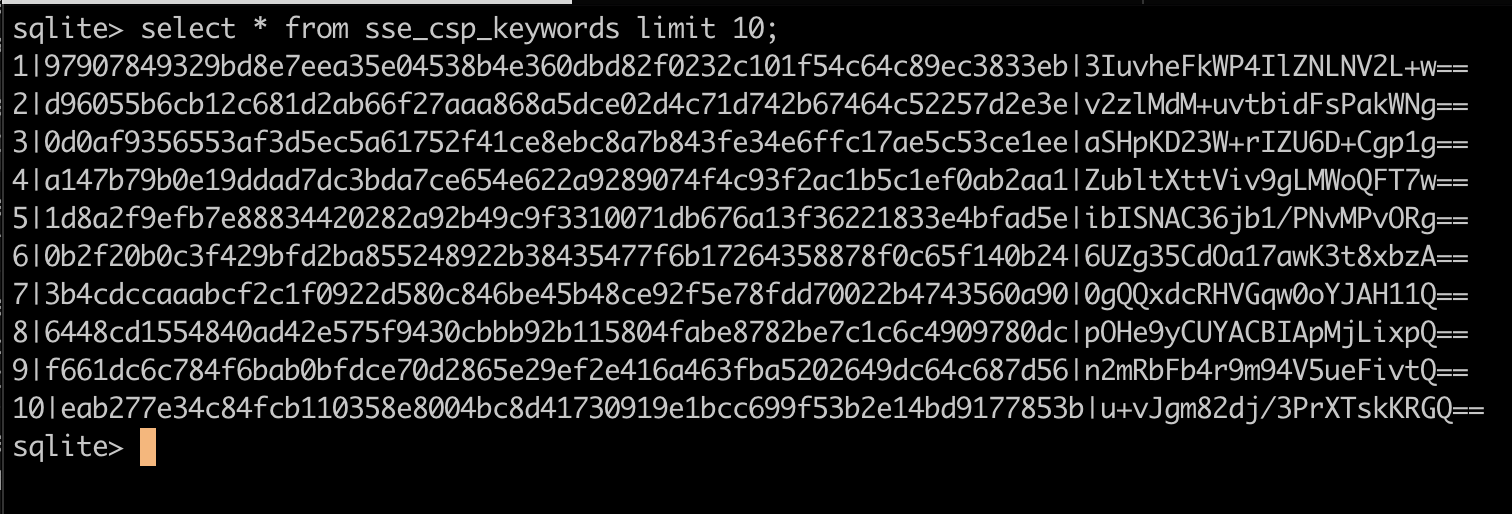
\includegraphics[height=\textheight,width=\textwidth,
    keepaspectratio]{sse_csp_keywords_table.png}
    \caption{sse\_csp\_keywords Table.}\label{fig:sse_csp_keywords}
\end{figure}

\begin{figure}[!hpt]
    \centering
    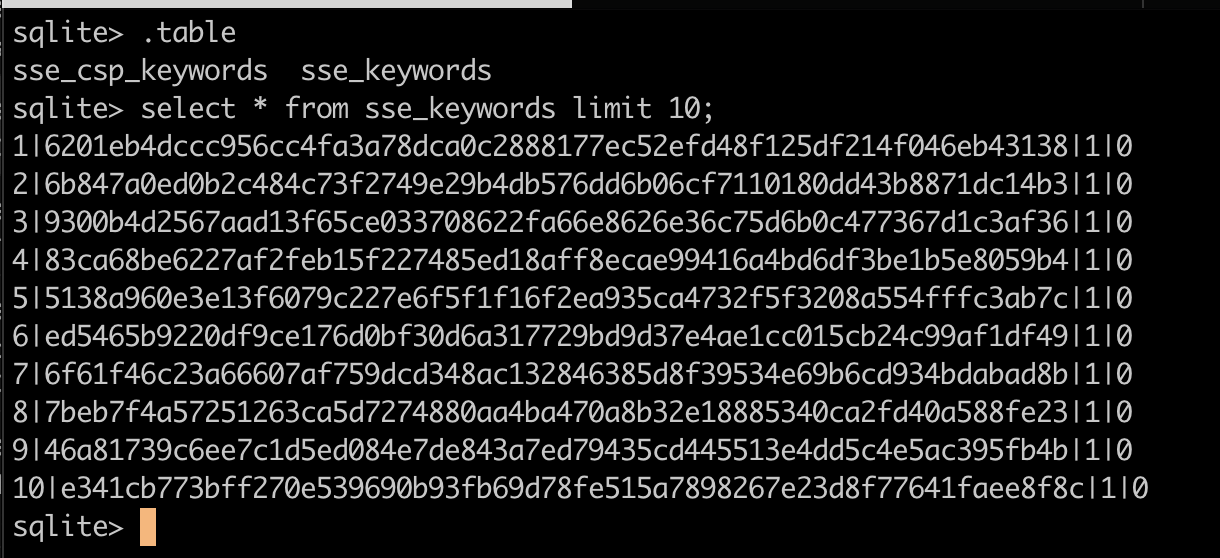
\includegraphics[height=\textheight,width=\textwidth,
    keepaspectratio]{sse_keywords_table.png}
    \caption{sse\_keywords Table.}\label{fig:sse_keywords}
\end{figure}

\textbf{Total combined size of test files: 136K --- 25 .txt files}.
It took around 1.89 seconds to create the dictionary and encrypt
25 .txt files (\autoref{fig:create_dict})

\begin{figure}[!hpt]
    \centering
    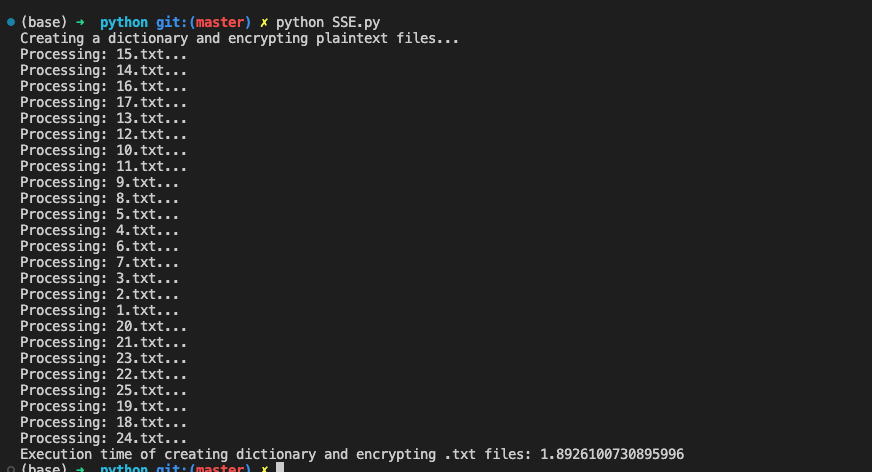
\includegraphics[height=\textheight,width=\textwidth,
    keepaspectratio]{create_dict_time_printing_included.png}
    \caption{Time taken to create the dictionary and encrypt 25 .txt files.}
    \label{fig:create_dict}
\end{figure}

\section*{Exercise 2 --- Searching in the dark}

\begin{figure}[!hpt]
    \centering
    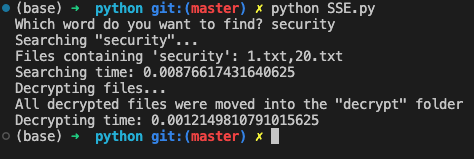
\includegraphics[height=\textheight,width=\textwidth,
    keepaspectratio]{searching_decrypting_time.png}
    \caption{Time taken to find the keyword and decrypt the files.}
\end{figure}

\begin{figure}[!hpt]
    \centering
    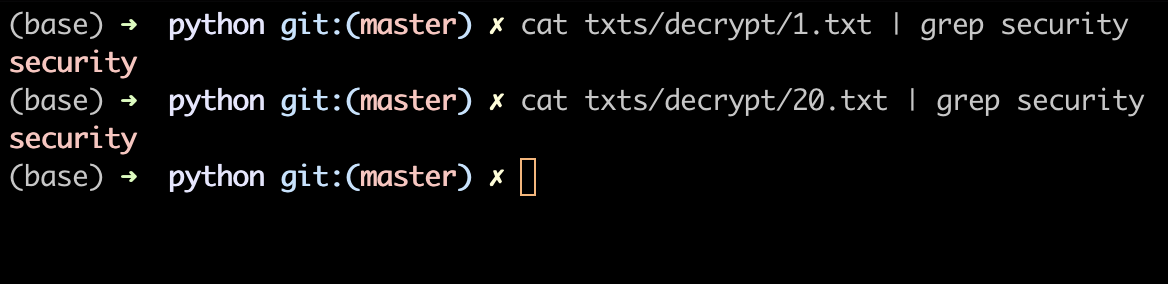
\includegraphics[height=\textheight,width=\textwidth,
    keepaspectratio]{keyword_in_decrypted_file.png}
    \caption{Keywords shown in decrypted .txt files.}
\end{figure}

\end{document}